% Prof. Dr. Ausberto S. Castro Vera
% UENF - CCT - LCMAT - Curso de Ci\^{e}ncia da Computa\c{c}\~{a}o
% Campos, RJ,  2022
% Disciplina: An\'{a}lise e Projeto de Sistemas
% Aluno:


\chapterimage{conclusoes.png} % Table of contents heading image
\chapter{Considera\c{c}\~{o}es Finais}


Desse modo, foi visado desenvolver um sistema para um \textit{Sistema remoto de gerenciamento de Carros Autônomos} de forma a encontrar todos os requisitos necessários suprindo as solicitações dos stakeholders .
O sistema atual para causara uma melhor transição e adaptação porém contendo todas as me- lhorias necessárias e atendendo seus requisitos, foram realizadas uma série de atividades, divididas em duas etapas: de planejamento e de análise. Seguindo o material bibliográfico do \cite{Dennis2014}.
Dentre as atividades realizadas estão o levantamento de requisitos, realização de entrevistas com stakeholders para melhor compreensão e priorização dos requisitos, estudo de casos de uso para o sistema, análise dos custos e benefícios do desenvolvimento deste novo sistema e um estudo sobre sua viabilidade. Concluiu-se que o sistema era viável e que seu desenvolvimento traria benefícios tanto tangíveis quanto intangíveis para a empresa.
Durante o cronograma estabelecido de um ano, serão desen- volvidos os sistemas remotos de gerenciamento dos veículos, assim como o aplicativo para os usuários.
 Esses sistemas podem também ser usados pelos seguintes stakeholders: funcionários, clientes e fornecedores e gerentes.

É de extrema importância salientar que o trabalho desenvolvido aqui serviu de aprendizado para o entendimento da disciplina de Análise e Projeto de Sistema. Deixo aqui meus sinceros agradecimentos ao professor, pela sua paciência e dedicação há nos alunos!



   \begin{figure}[H]
    \begin{center}
        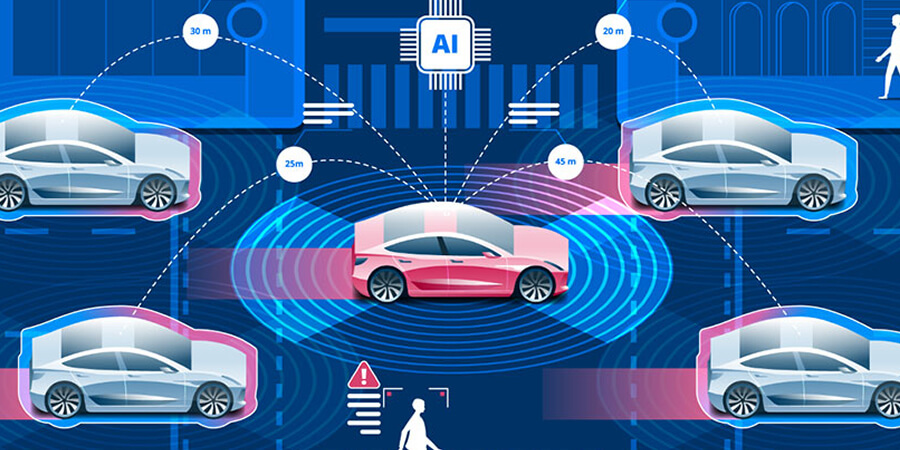
\includegraphics[width=12cm]{cars.jpg}
        \caption{Meu Sistema a ser desenvolvido} \label{sistema}
    \end{center}
   \end{figure}
